\section{Pristranskost podatkovnih baz}
Na vseh stopnjah raziskovanja in razvoja algoritmov razpoznavanja in detekcije objektov potrebujemo primerne podatkovne baze \cite{ponce2006dataset}. So glavni razlog za razvoj računalniškega vida, saj vsebujejo veliko podatkov za učenje, prav tako pa z njimi lahko primerjamo algoritme med seboj \cite{torralba2011unbiased}. Ravno zaradi podatkovnih baz lahko rečemo, da je računalniški vid ekspermentalna znanost \cite{torralba2011unbiased}. Čeprav si brez njih razvoja računalniškega vida težko predstavljamo, pa v njih obstajata dva temeljna problema, vedenjske napake in pristranskost. 

S podatkovnimi bazami se raziskovalci osredotočajo na premagovanje pogostokrat ene številke, ki predstavlja zmogljivost algoritma \cite{torralba2011unbiased}. Kot so pokazali v \cite{?}, bolj zmogljiv algoritem ni nujno statistično signifikanten.  Podatkovne baze, ki bi morale biti vzorec realnega sveta tako postanejo same sebi namen \cite{torralba2011unbiased}. Zadnji očiten vedenjski problem pa je t.i. plazeča prenasičenost, kot jo imenuje \cite{torralba2011unbiased}. Če je podatkovna baza dolgo na razpolago, algoritme že tako dobro nastavimo na bazo, da izgubi možnost generalizacije \cite{torralba2011unbiased}.

Še večji problem podatkovnih baz je njihova kvaliteta. V delih, ki jih bomo podrobneje predstavili v nadaljevanju, opisujejo ravno ta aspekt podatkovnih baz. Kvaliteta se najpogosteje odraža v pristranskosti podatkovnih baz in močno vpliva na algoritme. Lahko bi rekli, da je zmogljivost algoritma odvisna od kvalitete podatkovne baze, ki jo uporabljamo za razvoj. Seveda obstaja veliko pristranskosti na račun različnega namena podatkovnih baz \cite{torralba2011unbiased}. Nekatere vsebujejo samo prizore, druge profesionalne fotografije in tretje amaterske fotografije iz interneta. Četudi bi izločili namensko pristranskost, so v \cite{torralba2011unbiased} ugotovili, da v določeni meri pristranskost še vedno obstaja. To so pokazali na primeru avtomobilov. Caltech tako vsebuje avtomobile s stranskim pogledom, ImageNet pa večinoma športne avtomobile \cite{torralba2011unbiased}. Skozi zgodovino razvoja podatkovnih baz lahko vidimo, da je razvoj potekal večinoma tako, da so se z novimi podatkovnimi bazami hoteli znebiti pojavljajoče pristranskosti \cite{torralba2011unbiased}. Kljub trudu pristranskost ostaja.


V \cite{ponce2006dataset} so večinoma raziskovali Caltech 101 \cite{fei2007learning} in PASCAL VOC podatkovno bazo \cite{?}. Za Caltech 101 so poudarili, da ne obstaja medrazredna variabilnost. Večino objektov izbranega razreda ima enako velikost, orientacijo in zorni kot pogleda. To lahko enostavno prikažemo s povprečenjem slik izbranega razreda. Če bi imeli veliko variacijo, bi bile slike \ref{fig:} homogene.

\begin{figure}[!htbp]
	\centering
	\includegraphics[width=0.7\columnwidth]{ponce_1}
	\caption{}
\end{figure}

PASCAL VOC podatkovna baza, naj bi rešila probleme Caltech 101. Ima večjo medrazredno variabilnost, prav tako pa se pojavlja šum v ozadju in okluzija objektov \cite{ponce2006dataset}. Za zelo dobre metode so se pri tej podatkovni bazi izkazale tiste, ki iščejo globalno informacijo v sliki. To vodi v problem slabe generalizacije \cite{ponce2006dataset}. Modeli se lahko naučijo, da so avtomobili povezani s cesto in potem ne delujejo na primerih kjer je avto na polju. Na tak način ne vemo, ali algoritmi razpoznavajo objekt ali ozadje \cite{ponce2006dataset}.

V delu \cite{pinto2008why} so se prav tako osredotočali na podatkovno bazo Caltecch 101 \cite{fei2007learning}. Preverili so delovanje sistema V1. Sistem V1, temelji na Gaborjevih filtrih in predstavlja prvo procesno enoto v vidnem sistemu primatov \cite{pinto2008why}. Z zmogljivostjo \proc{67} je dokaj primitiven algoritem presegel večino do tedaj najboljših algoritmov. S tem so dokazali, da testiranje na tovrstnih naravnih slikah ni dovolj dobro. Predlagali so, da objektivno evaluacijo težavnosti nalog razpoznavanja preverjamo z t.i. ničtimi modeli. Podatkovne baze bi morale biti zelo velike in nepristranske, da bi zaobjeli čimvečjo populacijo. Zaradi težavnosti pridobivanja takih podatkovnih baz so predlagali uporabo sintetičnih slik.

S težavami modernejših podatkovnih baz so se ukvarjali v \cite{torralba2011unbiased}. S preprostim poskusom so najprej pokazali, da razvrščevalnik, ki razpoznava podatkovne baze deluje razmeroma dobro (\proc{39}). Z opazovanjem konfuzijske matrike, so ugotovili, da obstaja združevanje podatkovnih baz na tiste, ki se osredotočajo na prizore in tiste, ki se osredotočajo na objekte. Kljub majhnemu vzorcu je bila močno izražena diagonala, kar pomeni, da imajo podatkovne unikatne značilnosti \cite{torralba2011unbiased}. 

Nadalje so uvedli nov način testiranja zmogljivosti algoritmov z generalizacijo med bazami. S križnim testom so učili na eni bazi in testirali na drugi. Ker podatkovne baze predstavljajo vzorec naše realnosti, bi moral biti test za algoritme enostaven \cite{torralba2011unbiased}. Kot so pokazali, je pri testiranju z drugo podatkovno bazo zmogljivost algoritmov močno padla. Tako je na primeru razvrščanja avtomobilov padla iz \proc{53.4} na \proc{27.5} \cite{torralba2011unbiased}. Argumentirali so, da to nastane zaradi naslednjih razlogov \cite{torralba2011unbiased}:

\begin{enumerate}
	\item \emph{Pristranskost izbire}: Podatkovne baze preferirajo slike s specifičnimi lastnostmi.
	\item \emph{Pristranskost vzorčenja}: Ljudje fotografiramo objekte na podoben način.
	\item \emph{Pristranskost kategorij}: Semantične kategorije so slabo definirane in isti tipi objektov imajo lahko različne labele. 
	\item \emph{Pristranskost negativnega vzorca}: Representativnost negativnih primerov slik je slaba.
\end{enumerate}

Še posebej so poudarili, da ima največji vpliv \emph{pristranskost negativnega vzorca}. Če recimo želimo najti vse slike z avtomobili, kako vemo, da razvrčevalnik najde avtomobile in ne ceste, ki je s prevoznimi sredstvi močno korelirana \cite{torralba2011unbiased}? Tu pride prav negativni vzorec, v katerega damo primere cestišč in tako prisilimo algoritme v pravilno delovanje. S preizkusom na negativni množici primerov, združeni iz vseh baz, so v \cite{torralba2011unbiased} pokazali, da so negativni primeri iz različnih baz povezanimi s pozitivinimi primeri testne podatkovne baze (slaba reprezentativnost negativnih primerov).

Pomislili bi lahko, da bi se  z združevanjem podatkovnih baz rešili problematike pristranskosti. Vendar pa, kot so poudarili v \cite{torralba2011unbiased}, če želimo podatkovno bazo izboljšati, bi morali močno povečati učno množico, da bi bila ta signifikantna. Tako bi recimo za izboljšanje detektorja avtomobila na 1250 primerov PASCAL VOC 2007 morali dodati 50000 LabelMe vzorcev \cite{torralba2011unbiased}. 
Sama vrednost vrednost podatkovnih baz za delovanje algoritmov v resničnem svetu je tako po mnenju \citea{torralba2011unbiased}: ``boljša kot nič, vendar ne velika".

Problematika kako lahko uporabimo znane podatke za generalizacijo na še nepoznanih podatkih je v strojnem učenju poimenovana kot premostitev domen (angl. Domain Shift) \cite{tommasi2017deeper}. Domena je množica podatkov z lastno distribucijo glede na izbrane labele \cite{tommasi2017deeper}. Domene so tako lahko podatkovne baze ali resnični svet. Logično je, da algoritem lahko deluje v drugi domeni (nepoznana množica) samo v primeru, če dobro deluje v svoji bazični domeni (poznana množica podatkov) \cite{tommasi2017deeper}. Ker aspekta pri križnem testiranju med podatkovnimi bazami v \cite{torralba2011unbiased} niso upoštevali, so zato v \cite{tommasi2017deeper} predstavili novo metriko križnega testiranja generalizacije modelov. V \cite{torralba2011unbiased} so uporabili le relativno metriko
(procentualni upadec zmogljivosti), v \cite{tommasi2017deeper} pa so obravnavali delovanje tudi na učni množici z enačbo \eqref{eq:tommasi_1}, kjer je $s$ zmogljivost znotraj podatkovne baze in $o$ zmogljivost med podatkovnimi bazami. Vrednosti metrike se nahajajo na intervalu $[0,~1]$. Če je $CD$ večja od \num{0.5} nakazuje, da obstaja pristranskost. Vrednosti pod \num{0.5} pa govorijo o tem, da je $o \geq s$ ali pa so rezultati $s$ zelo nizki.  


\begin{equation}
	CD = \frac{1}{1+\exp\{-\frac{s-o}{100}\}}
	\label{eq:tommasi_1}
\end{equation}

Pri analizi pristranskosti ob uporabi DeCAF značilk so v \cite{tommasi2017deeper} dobili rezultate zmogljivosti večrazrednega razvrščanja, katerih povprečja so povzeta v tabeli \ref{tab:tommasi_1}. Vidimo lahko, da metrika $CD$ nakazuje na to, da imajo vse podatkovne baze približno enako pristranskost ne glede na izbiro značilke BOWSift ali DeCAF7. Po drugi strani pa z metriko upada vidimo večje razlike med podatkovnimi bazami.  

\begin{table}[!htbp]
	\centering
	\begin{tabular}{l S[table-format=1.3, round-mode=places, round-precision=2]  S[table-format=1.3, round-mode=places, round-precision=2]  S[table-format=1.3, round-mode=places, round-precision=2]  S[table-format=1.3, round-mode=places, round-precision=2]}
		\toprule
		& \multicolumn{2}{c}{\textbf{BOWSift}} & \multicolumn{2}{c}{\textbf{DeCAF7}} \\
		\cmidrule(lr){2-3} \cmidrule(lr){4-5}
		\textbf{Podatkovna baza} & \thead{Upad [\%]} & \theadm{CD} & \thead{Upad [\%]} & \theadm{CD} \\
		\midrule
		Caltech 256 & 51.5 & 0.53 & 47.9 & 0.58 \\
		ImageNet & 34.0  & 0.52 & 33.2 & 0.55 \\
		SUN & 42.1 & 0.51 & 25.9 & 0.52 \\
		\bottomrule
	\end{tabular}
	\caption{}
	\label{tab:tommasi_1}
\end{table}
